
\documentclass[a4paper]{article}
\usepackage{amsmath}

\usepackage{tikz}
\usetikzlibrary{bayesnet}


\begin{document}
\pagestyle{empty}

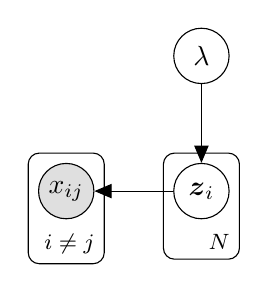
\begin{tikzpicture}
    \node[obs]                      (x_ij) {$x_{ij}$};
    \node[latent, right=of x_ij]                 (z)    {$\boldsymbol{z}_i$};
    \node[latent, above=of z]                    (lambda) {$\lambda$};

    \edge{lambda}{z};
    \edge{z}{x_ij}

    \plate{}{(x_ij)}{$i\neq j$};
    \plate{}{(z)}{$N$};
\end{tikzpicture}
\end{document}